\documentclass[11pt,a4paper]{article}
\usepackage[margin=2cm]{geometry}
\usepackage{graphicx}
\usepackage{amsmath,amssymb}
\usepackage{enumitem}
\usepackage{xcolor}
\usepackage{tcolorbox}
\usepackage{booktabs}
\usepackage{hyperref}
\usepackage{titlesec}
\usepackage{fancyhdr}

\definecolor{qcolor}{HTML}{1A5276}
\definecolor{acolor}{HTML}{196F3D}
\definecolor{seccolor}{HTML}{922B21}
\definecolor{boxbg}{HTML}{EBF5FB}
\definecolor{ansbox}{HTML}{EAFAF1}
\definecolor{tipbox}{HTML}{FEF9E7}

\tcbset{
    qbox/.style={colback=boxbg, colframe=qcolor, coltitle=white, fonttitle=\bfseries, coltext=black, left=4pt, right=4pt, top=4pt, bottom=4pt, boxrule=0.8pt, arc=3pt},
    abox/.style={colback=ansbox, colframe=acolor, coltitle=white, fonttitle=\bfseries, coltext=black, left=4pt, right=4pt, top=4pt, bottom=4pt, boxrule=0.5pt, arc=3pt},
    tipbox/.style={colback=tipbox, colframe=orange!70!black, fonttitle=\bfseries, left=4pt, right=4pt, top=4pt, bottom=4pt, boxrule=0.5pt, arc=3pt}
}

\newcounter{qcounter}
\newcommand{\vq}[1]{\stepcounter{qcounter}\begin{tcolorbox}[qbox, title=Q\theqcounter]#1\end{tcolorbox}}
\newcommand{\va}[1]{\begin{tcolorbox}[abox, title=Answer]#1\end{tcolorbox}\vspace{6pt}}

\pagestyle{fancy}
\fancyhf{}
\fancyhead[L]{\small\textbf{TFML Viva Prep — Part 1}}
\fancyhead[R]{\small CS6302E | Winter 2026}
\fancyfoot[C]{\thepage}

\title{\textbf{TFML Assignment Viva — Question Bank}\\[4pt]\Large Part 1: Problem Setup, Data, Architecture \& Training}
\author{CS6302E — Theoretical Foundations of Machine Learning}
\date{NIT Calicut | Winter 2026}

\begin{document}
\maketitle
\tableofcontents
\newpage

%=============================================================================
\section{Problem Statement \& Data Representation}
%=============================================================================

\vq{What is the problem you are solving in this assignment?}
\va{We are solving a \textbf{3-class pattern classification} problem. The task is to classify 8$\times$8 pixel images of the letters \textbf{B, 0 (zero), and E} using a single hidden-layer feedforward neural network trained from scratch with backpropagation.}

\vq{How are the letter templates represented numerically?}
\va{Each letter is an 8$\times$8 grid where \textbf{black (ink/stroke) pixels = $-1.0$} and \textbf{white (background) pixels = $+1.0$}. The template is then \textbf{flattened into a 64-dimensional vector} to serve as the input to the network.}

\vq{Why use $-1$ and $+1$ instead of $0$ and $1$ for pixel values?}
\va{Using $-1/+1$ (bipolar encoding) centers the data around zero, which helps with \textbf{gradient flow} during training. With $0/1$ encoding, inputs of $0$ contribute nothing to weight updates (since $0 \times \text{anything} = 0$), making learning slower. Bipolar encoding ensures every pixel \textbf{actively participates} in the weight update.}

\vq{How many total pixels does each input have, and why?}
\va{Each input has \textbf{64 pixels} ($8 \times 8 = 64$). The $8\times 8$ resolution is sufficient to capture the structural differences between B, 0, and E while keeping the input dimensionality small enough for a simple network.}

\vq{Show me the templates. How do B, 0, and E structurally differ?}
\va{
\begin{center}
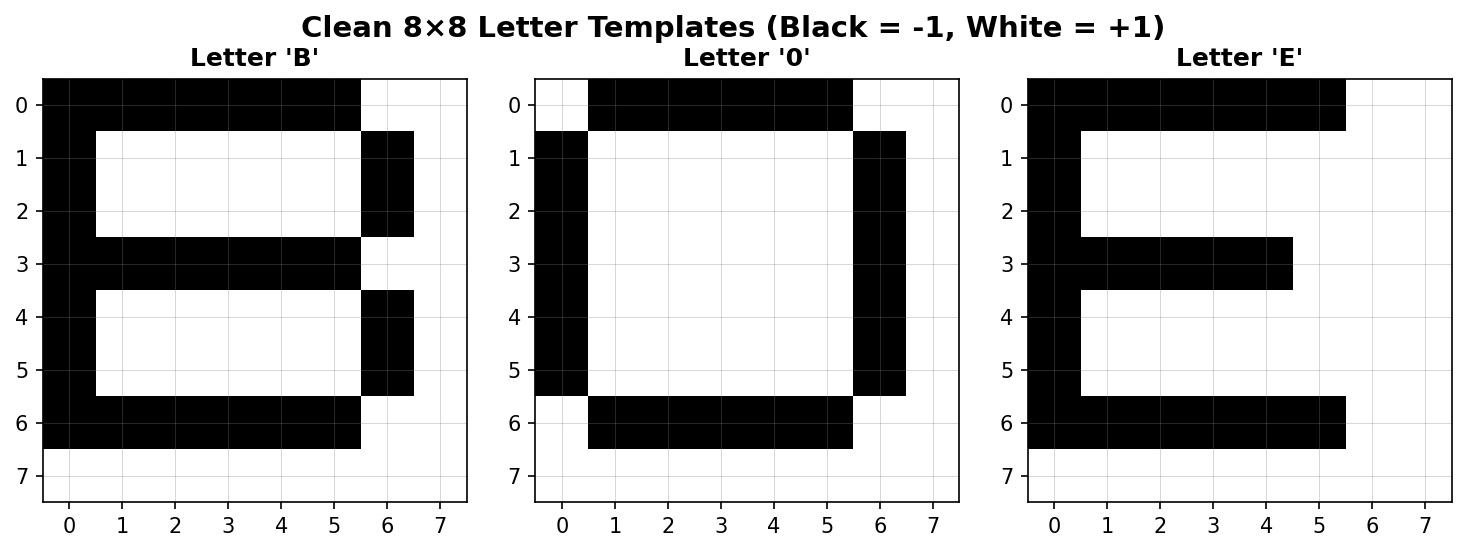
\includegraphics[width=0.85\textwidth]{templates.png}
\end{center}
\begin{itemize}[nosep]
    \item \textbf{B} has a vertical left bar, a middle horizontal bar, and two enclosed bumps on the right
    \item \textbf{0} has a closed loop — vertical bars on left and right, horizontal bars top and bottom, open center
    \item \textbf{E} has a vertical left bar and three horizontal bars (top, middle, bottom) but is \textbf{open on the right side}
    \item Key discriminators: B vs E — B has right-side enclosure; B vs 0 — B has a middle bar; 0 vs E — 0 has right vertical bar
\end{itemize}
}

%=============================================================================
\section{Noise \& Signal-to-Noise Ratio}
%=============================================================================

\vq{How is the noisy dataset generated?}
\va{For each of the 3 letters, we generate \textbf{100 noisy copies} by adding \textbf{independent uniform random noise from $U(-5, +5)$} to each of the 64 pixels. This produces a dataset $D$ of \textbf{300 total samples} (100 per class).}

\vq{What is the signal-to-noise ratio (SNR) in this problem?}
\va{The signal range is \textbf{2 units} (from $-1$ to $+1$), while the noise range is \textbf{10 units} (from $-5$ to $+5$). The noise range is \textbf{$5\times$ the signal range}, giving an SNR of approximately \textbf{$-14$ dB}. This is a very low SNR, meaning the noise is much stronger than the signal, making classification extremely challenging.}

\vq{Why use uniform noise instead of Gaussian noise?}
\va{Uniform noise $U(-5,+5)$ has a \textbf{bounded range} — every noise value is guaranteed to be within $[-5, +5]$. Gaussian noise has unbounded tails. Uniform noise provides a \textbf{controlled, worst-case noise scenario} where every noise value within the range is equally likely. The assignment specification required uniform noise.}

\vq{Look at the noisy samples. Can you visually identify the letters?}
\va{
\begin{center}
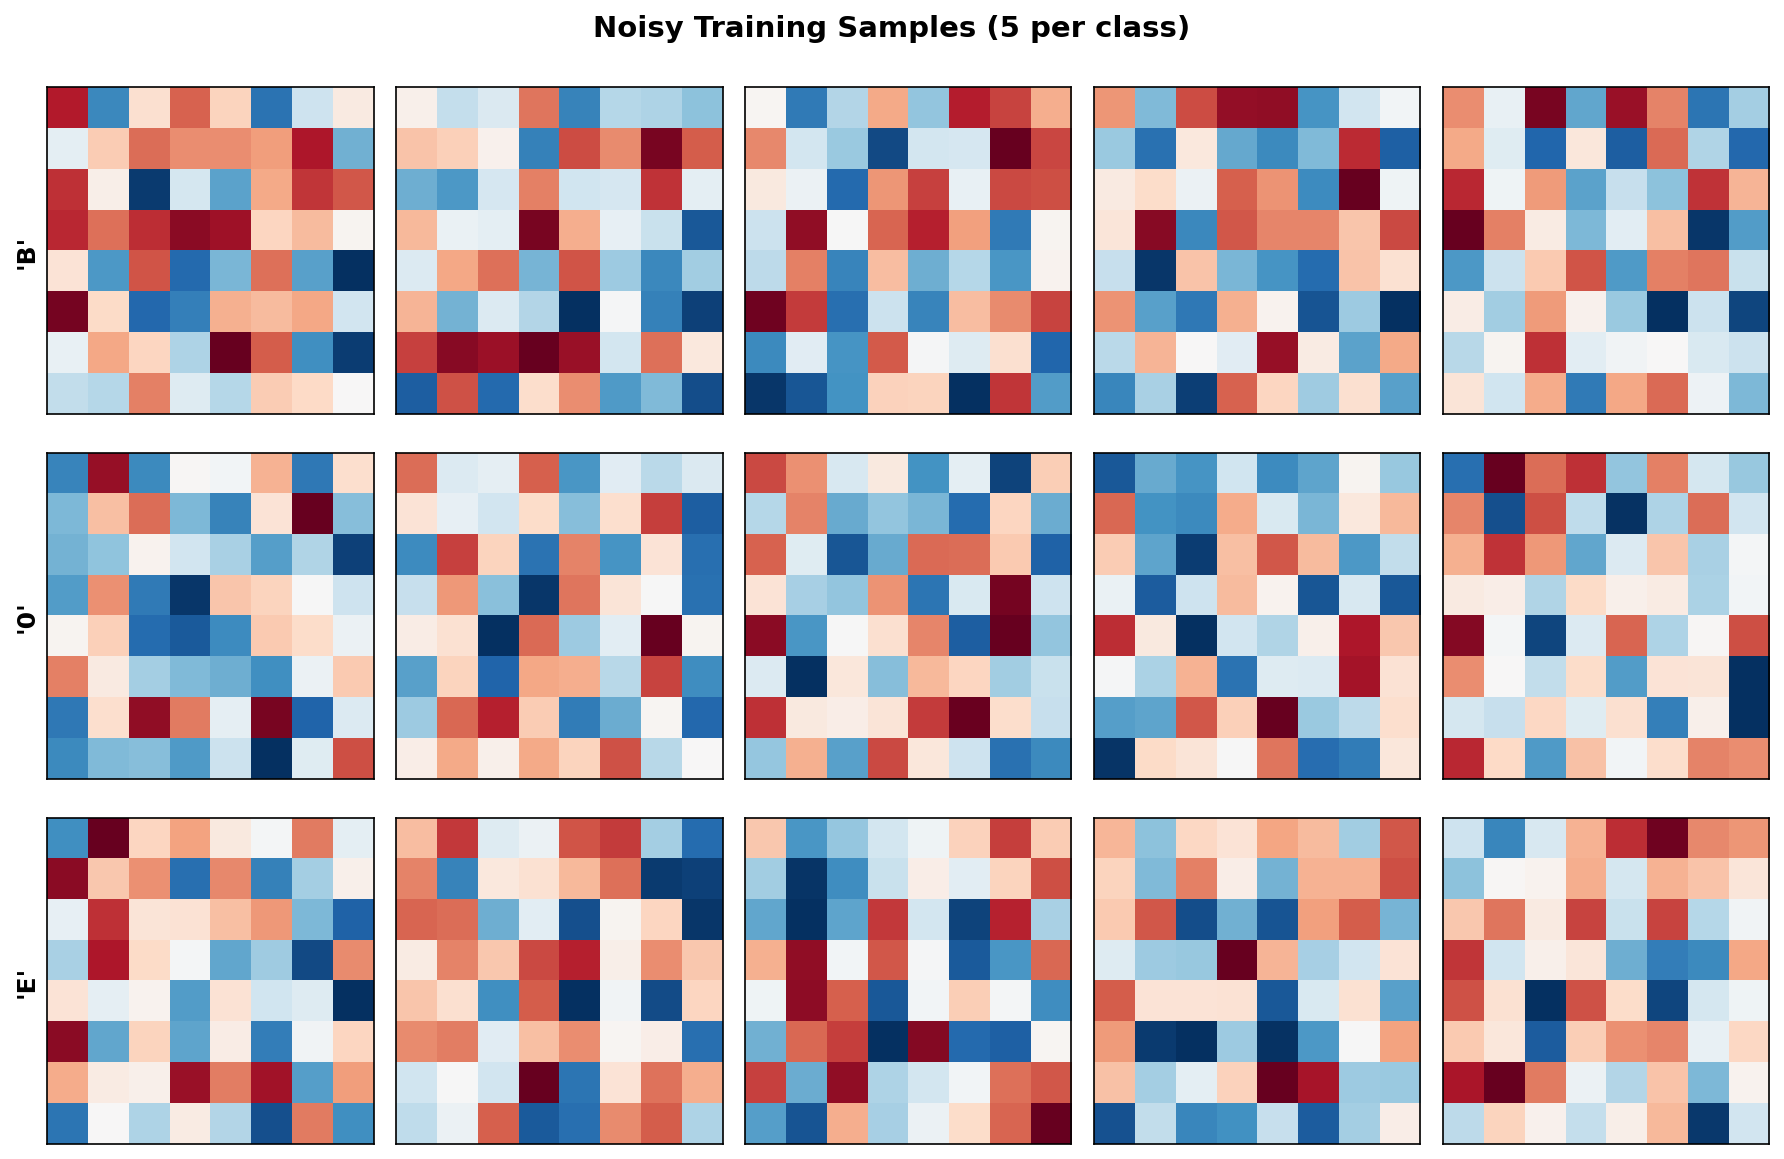
\includegraphics[width=0.80\textwidth]{noisy_samples.png}
\end{center}
No — the noisy samples are \textbf{visually indistinguishable} from random noise. The noise (range 10) completely overwhelms the signal (range 2). The network must learn to \textbf{average out the noise} across many training examples to find the underlying pattern.
}

\vq{What is the expected value and variance of a single noisy pixel?}
\va{For a pixel with true value $t$ (either $-1$ or $+1$):
\begin{itemize}[nosep]
    \item \textbf{Expected value} = $t + 0 = t$ (noise has zero mean)
    \item \textbf{Variance of noise} = $\frac{(5 - (-5))^2}{12} = \frac{100}{12} \approx 8.33$
    \item \textbf{Standard deviation} $\approx 2.89$ (larger than the entire signal range of 2)
\end{itemize}
}

\vq{With 100 samples per class, how does averaging help the network learn?}
\va{Since the noise has zero mean, averaging $N$ samples reduces the noise standard deviation by a factor of $\sqrt{N}$. With 100 samples, the effective noise is reduced by $\mathbf{10\times}$, bringing the effective SNR to a workable level. The weights converge to values proportional to the \textbf{expected (clean) pixel values}.}

%=============================================================================
\section{Neural Network Architecture}
%=============================================================================

\vq{Describe the architecture of the neural network (64-3-3).}
\va{It is a \textbf{single hidden-layer feedforward neural network} with:
\begin{itemize}[nosep]
    \item \textbf{Input layer}: 64 neurons (one per pixel)
    \item \textbf{Hidden layer}: 3 neurons with sigmoid activation
    \item \textbf{Output layer}: 3 neurons with sigmoid activation (one per class: B, 0, E)
    \item \textbf{Biases} included in both hidden and output layers
    \item Total parameters: $(64\times3 + 3) + (3\times3 + 3) = \mathbf{207}$
\end{itemize}
}

\vq{Why exactly 3 hidden neurons? Is this the minimum?}
\va{3 hidden neurons is the \textbf{theoretical minimum} for a 3-class classification problem. Each hidden neuron can learn to function as a specialized \textbf{feature detector}, and with 3 classes, you need at least 3 linearly independent feature representations to distinguish all classes.}

\vq{How many total trainable parameters does the 64-3-3 network have?}
\va{
\begin{itemize}[nosep]
    \item $W_1$ (input$\to$hidden): $64 \times 3 = 192$ weights
    \item $b_1$ (hidden biases): 3 biases
    \item $W_2$ (hidden$\to$output): $3 \times 3 = 9$ weights
    \item $b_2$ (output biases): 3 biases
    \item \textbf{Total: $192 + 3 + 9 + 3 = 207$ parameters}
\end{itemize}
}

\vq{What is the role of the hidden layer?}
\va{The hidden layer performs \textbf{feature extraction} — it transforms the raw 64-dimensional pixel input into a compact 3-dimensional \textbf{internal representation}. Each hidden neuron acts as a \textbf{feature detector} that responds to specific spatial patterns. The output layer then makes the classification decision based on these extracted features.}

\vq{Why is this a ``single hidden-layer'' network and not a deep network?}
\va{It has only \textbf{one layer of learned features} between input and output. The \textbf{Universal Approximation Theorem} states that a single hidden layer with enough neurons can approximate any continuous function. For this relatively simple 3-class task, one hidden layer suffices.}

\vq{Why use sigmoid activation and not ReLU or tanh?}
\va{Sigmoid maps values to $(0, 1)$, natural for class probabilities. For a TFML course, sigmoid is pedagogically important:
\begin{itemize}[nosep]
    \item Its derivative has a \textbf{simple closed form}: $\sigma'(z) = \sigma(z)(1-\sigma(z))$
    \item It demonstrates \textbf{vanishing gradient} issues clearly
    \item It's the classic activation in foundational neural network literature
\end{itemize}
}

%=============================================================================
\section{Activation Function Deep-Dive}
%=============================================================================

\vq{Write the sigmoid function and its derivative.}
\va{
\begin{align*}
    \text{Sigmoid:} \quad \sigma(z) &= \frac{1}{1 + e^{-z}} \\[4pt]
    \text{Derivative:} \quad \sigma'(z) &= \sigma(z) \cdot (1 - \sigma(z))
\end{align*}
If we already have $a = \sigma(z)$, the derivative is simply $a(1-a)$, which is computationally efficient.
}

\vq{What is the range of sigmoid? What happens at extreme values?}
\va{The range is $(0, 1)$ — it never reaches 0 or 1 exactly. As $z \to +\infty$, $\sigma(z) \to 1$. As $z \to -\infty$, $\sigma(z) \to 0$. At extreme values, the derivative approaches 0 (flat curve), causing the \textbf{vanishing gradient problem}.}

\vq{Why do you clip $z$ to $[-500, 500]$ in the sigmoid implementation?}
\va{To prevent \textbf{numerical overflow} in \texttt{exp(-z)}. When $z$ is very large negative (e.g., $-1000$), $e^{1000}$ overflows to infinity. Clipping to $[-500, 500]$ ensures numerical stability while having no practical effect on the output.}

\vq{What is the vanishing gradient problem and how does it relate to sigmoid?}
\va{The sigmoid derivative $\sigma'(z) = \sigma(z)(1-\sigma(z))$ has a \textbf{maximum value of 0.25} (at $z=0$). During backpropagation, gradients are multiplied by these derivatives layer by layer. With each layer, the gradient shrinks by at most $0.25\times$, causing gradients to \textbf{exponentially decay}. Less of a problem for our 2-layer network, but critical for deeper architectures.}

%=============================================================================
\section{Loss Function}
%=============================================================================

\vq{What loss function did you use and why?}
\va{\textbf{Mean Squared Error (MSE)}:
$L = \frac{1}{n}\sum(y_{\text{true}} - y_{\text{pred}})^2$

MSE is simple, differentiable, and its gradient is straightforward: $\frac{\partial L}{\partial y_{\text{pred}}} = y_{\text{pred}} - y_{\text{true}}$. For a TFML course, it demonstrates the fundamentals clearly.}

\vq{Why not use Cross-Entropy loss instead of MSE?}
\va{Cross-entropy would be more theoretically appropriate for classification because it measures the \textbf{divergence between probability distributions} and produces \textbf{stronger gradients} when wrong. However, MSE was used because: (1) simpler to derive/implement from scratch, (2) still works well, and (3) aligns with the foundational approach taught in TFML.}

\vq{How is MSE computed in your code?}
\va{\texttt{np.mean((y\_true - y\_pred) ** 2)} — computes the mean over \textbf{all samples AND all output neurons}. For 300 samples with 3 outputs each, it averages over 900 values.}

%=============================================================================
\section{Weight Initialization}
%=============================================================================

\vq{What weight initialization scheme did you use and why?}
\va{\textbf{Xavier/Glorot initialization}: weights drawn from $\mathcal{N}(0, \sqrt{2/(fan_{in} + fan_{out})})$.

For $W_1$: $\sqrt{2/(64+3)} \approx 0.173$. For $W_2$: $\sqrt{2/(3+3)} \approx 0.577$.

Xavier keeps the \textbf{variance of activations approximately constant} across layers, preventing exploding or vanishing activations during the forward pass.}

\vq{What would happen with random initialization from $\mathcal{N}(0,1)$?}
\va{The pre-activations would be \textbf{very large} (sum of 64 inputs $\times$ weights $\sim \mathcal{N}(0, 64)$), pushing sigmoid to extreme values (0 or 1). This causes \textbf{near-zero gradients} from the start (saturation), making training extremely slow or stuck. Xavier fixes this by scaling variance inversely with fan-in.}

\vq{How are biases initialized?}
\va{Biases are initialized to \textbf{zero}. This is standard — biases don't suffer from variance-scaling issues. The network breaks symmetry through the random weight initialization.}

%=============================================================================
\section{Training Procedure}
%=============================================================================

\vq{Describe the training procedure step by step.}
\va{
\begin{enumerate}[nosep]
    \item \textbf{Forward pass}: $a_1 = \sigma(X \cdot W_1 + b_1)$, then $a_2 = \sigma(a_1 \cdot W_2 + b_2)$
    \item \textbf{Compute MSE loss} between predicted output and one-hot targets
    \item \textbf{Backward pass}: Compute gradients of loss w.r.t.\ all weights and biases
    \item \textbf{Update weights}: $W \leftarrow W - \eta \cdot \partial L / \partial W$
    \item Repeat for \textbf{5000 epochs}
\end{enumerate}
}

\vq{What optimization algorithm did you use?}
\va{\textbf{Full-batch gradient descent} — the entire dataset of 300 samples is used to compute the gradient at each step. No mini-batches, no stochastic sampling. This gives the \textbf{exact gradient} but is only feasible for small datasets like ours.}

\vq{What is the learning rate and why that value?}
\va{Learning rate $\eta = 0.5$. Relatively high, works because full-batch gradient gives stable, non-noisy gradients; the problem is simple; and Xavier initialization ensures activations are in a good range.}

\vq{Why 5000 epochs? How did you decide this?}
\va{
\begin{center}
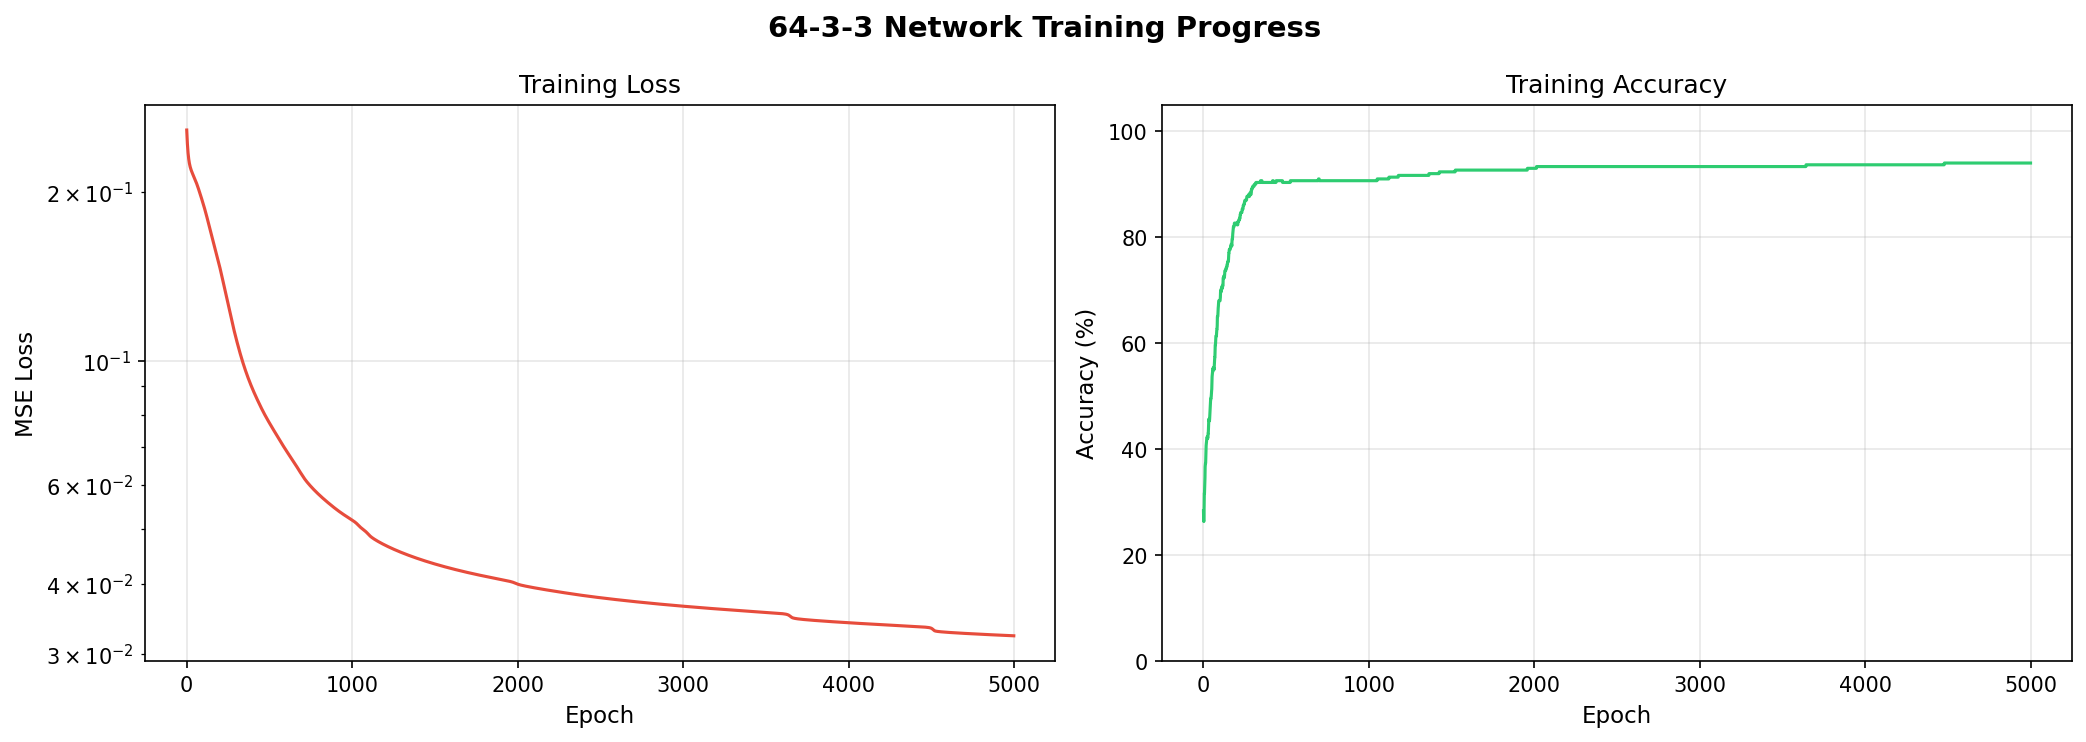
\includegraphics[width=0.85\textwidth]{training_curves.png}
\end{center}
From the training curves: most learning happens in the first 500--1000 epochs, then convergence slows. By epoch 5000, the loss has essentially plateaued at $\sim$0.03 and accuracy at $\sim$94\%. 5000 epochs ensures full convergence.
}

\vq{What does the log-scale loss curve tell you?}
\va{The log-scale reveals the \textbf{rate of convergence}. The initial steep drop (epochs 0--500) indicates rapid learning. The curve then transitions to a much slower decrease near a local minimum. The smooth, monotonic decrease confirms stable training with no oscillations.}

\vq{Why does accuracy jump in a step-like pattern while loss decreases smoothly?}
\va{Loss is \textbf{continuous} — it decreases smoothly as weights adjust. Accuracy is \textbf{discrete} — it only changes when a sample's predicted class flips. A sample's prediction can move closer to the decision boundary (loss decreasing) without crossing it (accuracy unchanged). When it crosses, accuracy jumps.}

\vq{What is the final training accuracy and what does it mean?}
\va{$\sim$\textbf{94\%} (282/300 correct). The 18 misclassified samples are so heavily corrupted by noise that they are closer to a different letter's template — these are \textbf{Bayes-irreducible errors} that no classifier can overcome.}

\begin{tcolorbox}[tipbox, title=\textbf{End of Part 1}]
\textbf{34 questions covered.} Continue to Part 2 for backpropagation math, confusion matrix analysis, and weight visualizations.
\end{tcolorbox}

\end{document}
